\documentclass[a4paper, 12pt]{article}

\newcommand{\bold}{\textbf}

\usepackage[english]{babel}
\usepackage{amsmath}
\usepackage{tikz}
\usepackage{indentfirst}

\begin{document}

\newcommand{\q2}{\quad\quad}

\title{\Large{\bold{Moontorio}}}
\author{Matei Adriel}
\date {}

\maketitle

\section{Example 1}

Solve the following factory:

\vspace*{20pt}
\begin{figure}[h]
\centering
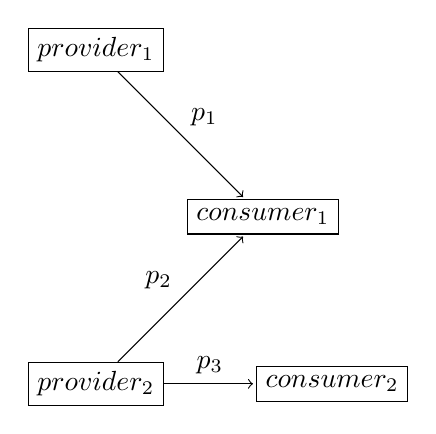
\begin{tikzpicture}[shorten >=1pt, auto, node distance={30mm}, 
  main/.style = {draw, rectangle}]

\node[main] (3) {$consumer_1$};
\node[main] (1) [above left of=3] {$provider_1$};
\node[main] (2) [below left of=3] {$provider_2$};
\node[main] (4) [right of=2] {$consumer_2$};

\draw[->] (1) edge node{$p_1$} (3);
\draw[->] (2) edge node{$p_2$} (3);
\draw[->] (2) edge node{$p_3$} (4); 

\end{tikzpicture}
\caption{Factory} 
\label{fig:Factory}
\end{figure}

Generating the constraints: 
\begin{figure}[h]
\centering

\begin{equation}
  p_1(t) < provider_1(t)
\end{equation}

\begin{equation}
  p_3(t) < consumer_2(t)
\end{equation}

\begin{equation}
\begin{split}
  \begin{cases}
    \begin{cases}
      p_2(t) &< \displaystyle\frac{consumer_1(t)}{2}\\
      p_1(t) &< consumer_1(t) - p_2(t)
    \end{cases}
    \ ,&\;\mbox{if } p_1(t) \geq p_2(t)\\\\
    \begin{cases}
      p_1(t) &< \displaystyle\frac{consumer_1(t)}{2}\\
      p_2(t) &< consumer_1(t) - p_1(t)
    \end{cases}
    \ ,&\;\mbox{if } p_1(t) < p_2(t)
  \end{cases}
\end{split}
\end{equation}

\begin{equation}
\begin{split}
  \begin{cases}
    \begin{cases}
      p_3(t) &< \displaystyle\frac{provider_2(t)}{2}\\
      p_2(t) &< provider_2(t) - p_3(t)
    \end{cases}
    \ ,&\;\mbox{if } p_2(t) \geq p_3(t)\\\\
    \begin{cases}
      p_2(t) &< \displaystyle\frac{provider_2(t)}{2}\\
      p_3(t) &< provider_2(t) - p_3(t)
    \end{cases}
    \ ,&\;\mbox{if } p_2(t) < p_3(t)
  \end{cases}
\end{split}
\end{equation}

\caption{Constraints}
\label{fig:Constraints}
\end{figure}

\end{document}
